\subsection{Analysis of tests}

The two tests were carried out in a classroom setting in two different courses, Advanced Programming and Frameworks and Architectures for the Web. All students in each class were given the pretest and the posttest, and used a CRS system in between. The Advanced Programming course used Mentimeter, and have done so throughout the semester. The Frameworks course used our system, CRSFIT, and have not used any other CRS throughout the semester. 
There were 10 students present while performing the tests in the Frameworks course. This resulted in 8 responses in the pretest (N = 8), and 10 in the posttest (N = 10). The pretest was send out to students before class, and they were given 5 minutes to answer it first if they had not done so already. 

There were 50 students presenent while performing the tests in the Advanced Programming course. This resulted in 48 responses in the pretest (N = 48) and 50 in the posttest (N = 50). Again we see more answering the posttest compared to the pretest. The pretest is substantially longer than the posttest, which could be a reason for the different amount of respondents in the first compared to the latter. In the Advanced Programming course, the pretest was carried out almost immediately, so people showing up late could also be a possible reason.


% Pretest, mean of individual and general interactivity
Within the pretest we asked students about \emph{Individual interactivity} and \emph{General interactivity}. The individual interactivity for both tests is shown in figure \ref{fig:individual_interactivity}. When students are asked to assess their own interactivity they tend to rate it lower than when they are asked to asses others in the general interactivity. The average for individual interactivity was 5,8 compared to 6,1 for the general interactivity. A similar measurement was found by \citeA[p.~400]{siau2006use} where they found 6.1 and 6.3 based on the same scale respectively for individual and general interactivity. 
%They also asked into individual and general interactivity again after implementing a CRS into a class and found that the students assessed the individual and general level higher (6.8 and 7.1 respectively). Side 400. Statistisk signifikant. Til diskussion. 

 \begin{figure}[H]
  \centering
     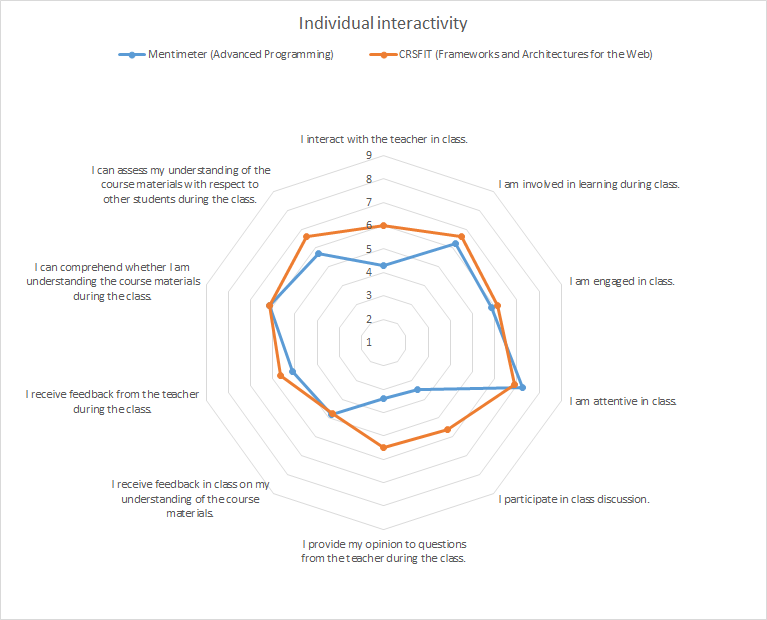
\includegraphics[width=\textwidth]{./individual_interactivity.png}
     \caption{\emph{Pretest - Individual Interactivity.}}
     \label{fig:individual_interactivity}
 \end{figure}

The individual interactivity shows if students believe they are active during a lecture. Both the Advanced and Frameworks course had two hours of lecture, and two hours of lab support. Figure \ref{fig:individual_interactivity} shows the similarities and differences in course participation. The biggest difference is found in the questions \emph{I participate in class discussion} and \emph{I provide my opinion to questions from the teacher during the class}. These questions are very specific to taking part in class and actively participating. Reasons for this could be found in the course differences. Advanced programming has formal prerequisites where you must be able to program, know basic functional programming and more. The Frameworks course is a introductory course and has no formal prerequisites. It is safe to assume that the learning curve is steeper in the Advanced Programming course, and therefore less people might participate in class discussions for example. Also course size might have influenced the outcome. The Advanced Programming course is over twice as large as the Frameworks course (42 vs 89), here students might hold back participation due to the large amount of people or there simply may not be time to have all students participate.

The general interactivity shows how students think others interact during a lecture. Compared to the individual interactivity the results here are much more aligned, as mentioned above. The highest differences are found in questions \emph{Students interact with the teacher in class} and \emph{Students are involved in learning during class}, but even here the interval between each are less than 1, and we do not deem this as a significant difference. Overall it would seem that the attitude towards general interactivity is very close to each other in the test. 

 \begin{figure}[H]
  \centering
     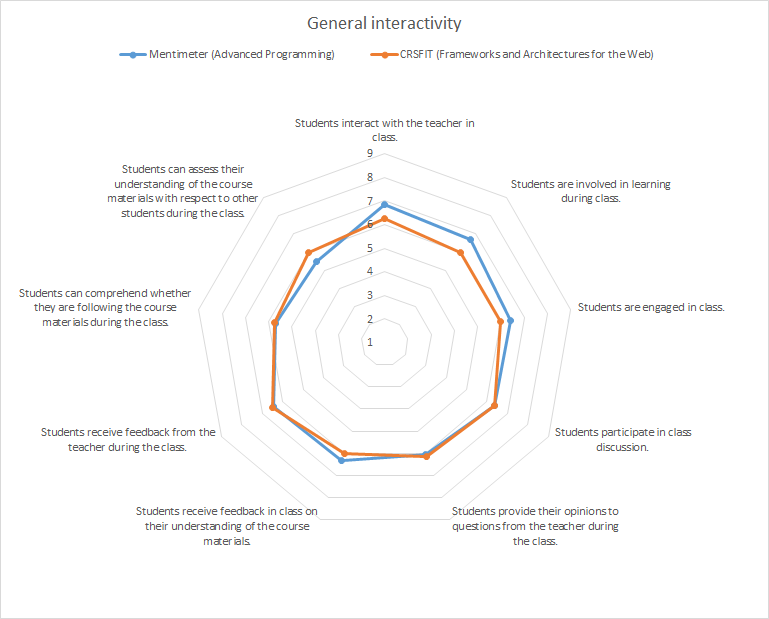
\includegraphics[width=\textwidth]{./general_interactivity.png}
     \caption{\emph{Pretest - General Interactivity.}}
     \label{fig:general_interactivity}
 \end{figure}


% Posttest, mean of Ease of use	and Perceived usefulness
In the posttest we asked the students to assess the \emph{ease of use} and \emph{perceived usefulness} of the CRS they were using. The overall mean of ease of use for CRSFIT is 7,8 and for perceived usefulness it is 6,7, compared to Mentimeters 8,1 and 8,3 respectively.

The relatively high value of ease of use suggests that the students found CRSFIT easy to use to an extend that is comparable to Mentimeter. The lower level of perceived usefulness could be explained by the way the test was carried out. The results may have been different if the test was carried out over a longer period of time in normal lectures. For example, students might be more convinced that a CRS is useful if they have used it over the course of a semester, and therefore rate the perceived usefulness higher. This is compared to testing CRSFIT in just one lecture, where the system is new to them.

We did expect the result would be closer to a more neutral 5 when we asked the students to assess how useful the system was. None of the students have seen the system before the test and the test was carried out in a little over half an hour. 

 \begin{figure}[H]
  \centering
     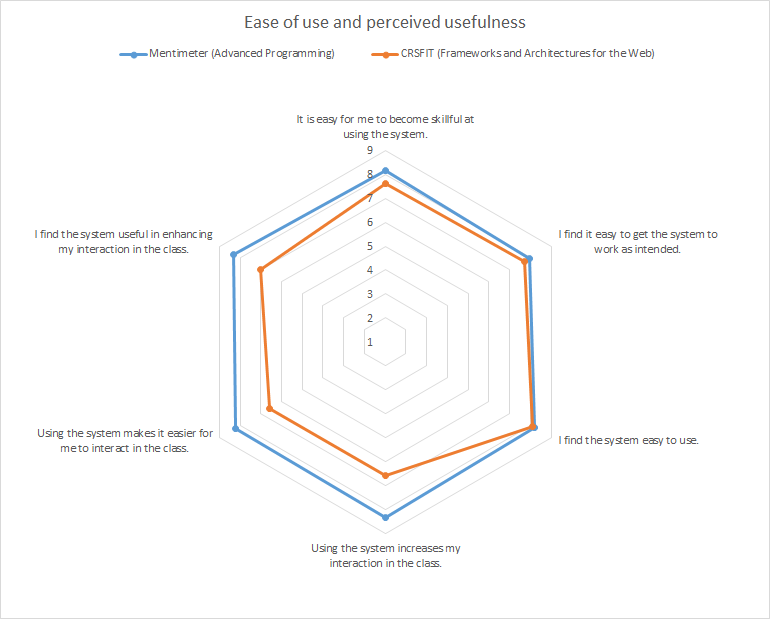
\includegraphics[width=\textwidth]{./perceived_ease_of_use_and_usefulness.png}
     \caption{\emph{Posttest - Ease of use and perceived usefulness.}}
     \label{fig:perceived_ease_of_use_and_usefulness}
 \end{figure}








% (M = 3.69, SD = 1.28) Mean, Standard Deviation

% individual vs. general -> I Individual er folk meget tilbageholdende 'nej vi siger ikek så meget, kunne godt deltage mere', men i general er de meget mere enige om at de alle deltager. Sjov udvikling :P 



 
 
















\subsubsection*{Qualitative part of the test}
In the posttest we asked both students from \emph{Advanced Programming} and \emph{Frameworks and Architectures for the Web} into the advantages and disadvantages of using a classroom response system. While the students from Advanced Programming used Mentimeter their comments must be seen in relation to this. The Advanced Programming course has been using Mentimeter from the very beginning of the semester, so they may have more experience with classroom response systems in general. The overall picture from the comments is that the students from Advanced Programming seems pleased with the system. One student points out a disadvantage when saying \emph{"Disadvange could be that people might not get the help they need during Classes."} (appendix \ref{app:qualitative-advanced}, item 25). If the time using a CRS is taken from helping students, then it's a clear disadvantage. However, it will always be the individual teacher's responsibility to manage the time in the courses they teach. Another student mentions awkward pauses when using Mentimeter (\ref{app:qualitative-advanced}, item 13). This may be the same for every CRS and it depends on how the teacher uses the system.

Among many of the advantages reported by the respondents from Advanced Programming is an increased attention, more interaction (\ref{app:qualitative-advanced}, item 4, 6, 10, 12, 13, 14) and forced thinking with feedback (\ref{app:qualitative-advanced}, item 11, 16, 17, 19, 20, 22). These advantages are just some of the advantages any CRS should provide when used properly. The overall picture from Advanced Programming seem that they found Mentimeter useful, which is also the picture we get when looking at the diagram in Figure \ref{fig:perceived_ease_of_use_and_usefulness}, where they report an average score bigger than 8. This is a better score than the one reported by the students from Frameworks and Architectures for the Web. Their comments somewhat reflect that as well, where they tend to be about the situation in which the test was carried out (\ref{app:qualitative-framworks}, item 1-4).

As highlighted by some of the respondents in the posttest from Frameworks and Architectures for the Web, there's room for improvement when using CRSFIT. The way the test was carried out didn't resemble a normal lecture. As mentioned earlier in chapter \ref{sec:testingcrs}, teaching and using a CRS requires training and experience. The test of the system was not carried out in a normal lecture by a teacher as it would have been if it was a normal setting. The test was carried out by us, letting people answer one question at a time. Normally, a teacher might ask one or two questions after a period of time or after finishing a subject and not ten questions at a time as it was the case in our test.

Two respondents answer that they would like to wait before seeing what other students answered. As one points out: \emph{"Students are easily biased, and it is hard to not look at what everyone else has answered before answering yourself."} (\ref{app:qualitative-frameworks}, item 4). We will not deny that and we may have seen biased answers in our test. For most questions in the test, the majority answered the correct answer except for the very last question. This particular question was made harder and more comprehensive. See appendix \ref{app:questions} item 10. The question got 8 responses and only two of them were correct. This may be because one of the first to answer answered incorrect and most people just followed along due to the difficulty of the question. So the respondents saying to wait some time before revealing answers would be better may have point. If we waited some time before showing what people answered, we would maybe have seen a more even spread in answers or maybe more correct answers in questions like the last one because students would individually take the time to figure out the answer. 

One respondent points out that the system de-personalizes the connection between teacher and student and another says it results in less individual feedback (\ref{app:qualitative-frameworks}, item 3 and 4). This was correct in our setting. A teacher may go more into detail why one answer is correct and another isn't. Maybe a teacher would ask the students why an answer is (in)correct and use the system to start a discussion. This way the personal connection could be maintained for people who are used to interact in class while people not used to interact in class would be included as well through the system.

One comment states that \emph{"it really helps examining yourself and seeing what you got or didn't get- at real time."} (\ref{app:qualitative-frameworks}, item 1). If students using our system immediately sees this advantage then we've come far. All of our questions were centered around topics covered in the course \emph{Frameworks and Architectures for the Web} in which our test was carried out. All of the questions and answers included code in a few different ways and we aimed at asking questions which they should be able to answer if they had followed the course. The comment implies we did that. 


